% *********************************************************************
% © 2021-2022 Jeremy Sylvestre
%
% Permission is granted to copy, distribute and/or modify this document
% under the terms of the GNU Free Documentation License, Version 1.3 or
% any later version published by the Free Software Foundation; with no
% Invariant Sections, no Front-Cover Texts, and no Back-Cover Texts. A
% copy of the license is included in the appendix entitled “GNU Free
% Documentation License” that appears in the output document of this
% PreTeXt source code. All trademarks™ are the registered® marks of
% their respective owners.
%
% *********************************************************************

\newcommand*{\xmin}{-0.25}
\newcommand*{\xmax}{5}
\newcommand*{\ymin}{-0.25}
\newcommand*{\ymax}{6.5}
\newcommand*{\func}{5 * \x - \x * \x}

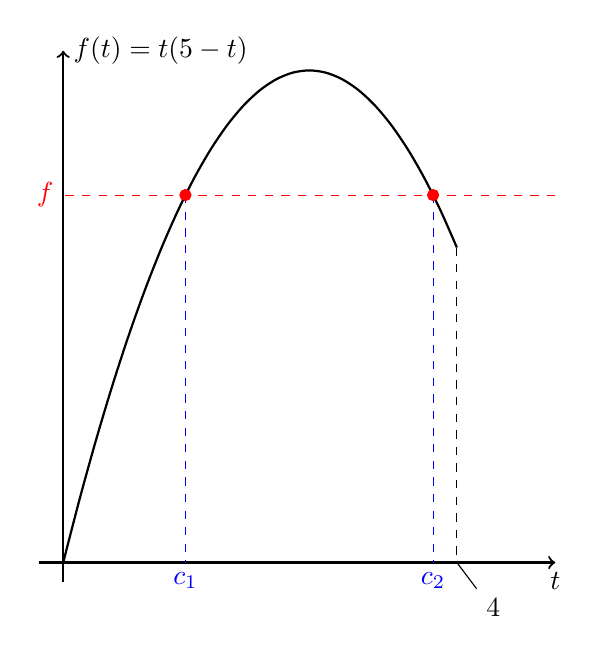
\begin{tikzpicture}
[
	closedpt/.style={circle,draw,fill,inner sep=0pt,minimum size=4pt},
	openpt/.style={circle,draw,inner sep=0pt,minimum size=4pt},
	xscale=1.25
]

	\draw[dashed] (4,4) to (4,0);
	\draw[thin] (4,0) -- (4.2,-0.333) node[below right] {$4$};

	% axes
	\draw[->,thick] (\xmin,0) -- (\xmax,0) node[below] {$t$};
	\draw[->,thick] (0,\ymin) -- (0,\ymax) node[right] {$f(t) = t (5 - t)$};

	% graph
	\draw[thick, domain=0:4, smooth] plot (\x,{\func});

	\draw[dashed,red] (\xmax,4.667) -- (0,4.667) node[left] {$\avg{f}$};
	\draw[dashed,blue] (1.242,4.667) -- (1.242,0) node[below] {$c_1$};
	\draw[dashed,blue] (3.758,4.667) -- (3.758,0) node[below] {$c_2$};

	\node[red,closedpt] at (1.242,4.667) {};
	\node[red,closedpt] at (3.758,4.667) {};

\end{tikzpicture}
